%%%%%%%%%%%%%%%%%%%%%%%%%%%%%%%%%%%%%%%%%%%%%%%%%%%%%%%%%%%
% --------------------------------------------------------
% Tau
% LaTeX Template
% Version 2.4.4 (28/02/2025)
%
% Author: 
% Guillermo Jimenez (memo.notess1@gmail.com)
% 
% License:
% Creative Commons CC BY 4.0
% --------------------------------------------------------
%%%%%%%%%%%%%%%%%%%%%%%%%%%%%%%%%%%%%%%%%%%%%%%%%%%%%%%%%%%

\documentclass[9pt,a4paper,twocolumn,twoside]{tau-class/tau}
\usepackage[portuguese]{babel}
%% Spanish babel recomendation
% \usepackage[spanish,es-nodecimaldot,es-noindentfirst]{babel} 
%% Draft watermark
% \usepackage{draftwatermark}
%----------------------------------------------------------
% TITLE
%----------------------------------------------------------

\journalname{Relatório de Sistema de Controle 1 - Engenharia de Computação}
\title{Controle de Posição em Sistema Massa-Mola com Conexão Flexível}

%----------------------------------------------------------
% AUTHORS, AFFILIATIONS AND PROFESSOR
%----------------------------------------------------------

\author[a,1]{Rafael Anacleto Alves de Souza}
\author[a,2]{Elvis Correia Lopes dos Santos}
\author[a,3]{Guilherme de Oliveira Costa}
%\author[a,4]{Pedro de Carvalho Cedrim}


%----------------------------------------------------------

\affil[a]{Instituto de Computação, Universidade Federal de Alagoas – Campus A.C. Simões\\
\textsuperscript{1}\texttt{raas@ic.ufal.br}, 
\textsuperscript{2}\texttt{ecls@ic.ufal.br}, 
\textsuperscript{3}\texttt{goc@ic.ufal.br}}
%\textsuperscript{4}\texttt{pcc@ic.ufal.br}}

\professor{Prof. Dr. Icaro Bezerra Queiroz de Araujo}

%----------------------------------------------------------
% FOOTER INFORMATION
%----------------------------------------------------------

\institution{Instituto de Computação, Universidade Federal de Alagoas}
%\footinfo{Relatório elaborado com classe \LaTeX\ Tau}
\theday{setembro de 2025}
\leadauthor{Souza, Santos e Costa}
\course{Engenharia de Computação - Sistemas de Controle 1}

%----------------------------------------------------------
% ABSTRACT AND KEYWORDS
%----------------------------------------------------------

\begin{abstract}    
    O projeto tem como objetivo o estudo e implementação de um sistema de controle de posição em uma configuração massa-mola com duas massas acopladas por molas, representando situações práticas de sistemas com ligação elástica entre atuador e carga.
   
    O problema central consiste em manter a posição controlada da massa de saída, mesmo diante das oscilações e acoplamentos internos do sistema. Para isso, pretende-se desenvolver um modelo matemático e realizar simulações computacionais.

    O foco é a obtenção do modelo matemático que descreve a dinâmica do sistema e sua simulação em malha aberta, servindo de base para o projeto e implementação do controlador de posição.
\end{abstract}

%----------------------------------------------------------

\keywords{sistema massa-mola, controle de posição, acoplamento elástico, resposta dinâmica, two-mass system}

%----------------------------------------------------------

\begin{document}
		
    \maketitle 
    \thispagestyle{firststyle} 
    \tauabstract
    % \tableofcontents
    % \linenumbers 
    
%----------------------------------------------------------

\section{Introdução}

\taustart{O}sistema massa-mola é um modelo físico clássico utilizado no estudo da dinâmica de sistemas oscilatórios. Consiste, em sua forma básica, em uma ou mais massas conectadas a molas, cuja força restauradora é descrita pela Lei de Hooke. Devido à sua simplicidade e capacidade de representar uma ampla gama de comportamentos dinâmicos, esse sistema é amplamente utilizado como base para a modelagem, simulação e controle de sistemas mecânicos reais.

Além do seu valor acadêmico, o modelo massa-mola possui diversas aplicações práticas. No setor automotivo, por exemplo, sistemas de suspensão utilizam molas para absorver impactos e estabilizar veículos. Em ambientes industriais, molas são aplicadas em dispositivos de medição, sistemas de amortecimento e na estabilização de estruturas. Dessa forma, compreender o comportamento desse tipo de sistema permite extrapolar conceitos para o desenvolvimento e controle de sistemas mais complexos.

O objetivo deste trabalho é o desenvolvimento de um sistema de controle para um protótipo massa-mola de configuração vertical. O sistema é composto por duas massas em cascata: a primeira massa ($M_1$) é suspensa por uma mola ($K_1$) e acoplada à segunda massa ($M_2$) por uma segunda mola ($K_2$). O controle de posição da massa inferior ($M_2$) é realizado por um servo motor, que atua na parte superior do sistema, e monitorado por um sensor a laser. Para atingir este objetivo, o projeto engloba a derivação do modelo matemático que descreve a dinâmica do sistema, a análise de seu comportamento por meio de simulação computacional e a posterior construção do protótipo físico para validação experimental.

\section{Descrição do Sistema}

O sistema proposto neste projeto adota uma configuração vertical com duas massas acopladas, montadas em um arranjo em cascata. A primeira massa ($M_1$) é suspensa por uma mola ($K_1$). O ponto de suspensão desta mola é movimentado verticalmente por um sistema de engrenagem e correia, acionado por um servo motor (modelo DS3230MG). Esta primeira massa está acoplada à segunda massa ($M_2$) por uma mola de ligação ($K_2$), deixando $M_2$ suspensa. A rotação do motor atua no conjunto superior, provocando o deslocamento vertical de todo o sistema.

O objetivo do controle é a posição da massa inferior ($M_2$), que é medida continuamente por um sensor a laser posicionado na base da estrutura. 

Para evitar interferências mecânicas e vibrações laterais indesejadas, as massas são fixadas em carrinhos que deslizam ao longo de um trilho vertical. Esta configuração atua como um guia linear, restringindo o movimento transversal para garantir uma trajetória puramente vertical. O atrito gerado pelo deslizamento dos carrinhos no trilho é o principal componente do atrito viscoso ($b_1$ e $b_2$) considerado no modelo matemático.

A montagem do sistema foi pensada para minimizar problemas comuns em estruturas horizontais, como o atrito entre a base e os elementos móveis. A disposição vertical também facilita a análise do sistema em termos de energia potencial, amortecimento e resposta transitória sob a atuação da gravidade.

%figura 1 - modelo massa mola montado

\section{Revisão Bibliográfica}

O sistema massa-mola é um modelo físico fundamental que descreve a interação entre uma massa e um dispositivo elástico, sendo central para o entendimento de fenômenos como oscilações e ondas. A dinâmica do sistema é governada pela Lei de Hooke, que estabelece que a força restauradora da mola é diretamente proporcional à sua deformação, agindo na direção oposta a ela. Quando o sistema é colocado em movimento, ocorre uma conversão contínua entre a energia potencial elástica, armazenada na deformação da mola, e a energia cinética, associada ao movimento da massa. Em sistemas reais, forças dissipativas como o atrito e a resistência do ar podem reduzir a amplitude, um fenômeno conhecido como amortecimento. \cite{SistemaMassaMola}

Em muitas aplicações industriais, como máquinas-ferramenta, braços robóticos flexíveis e laminadores de aço, a simplificação do modelo para uma única massa é inadequada, levando a um desempenho de controle insatisfatório. Isso ocorre especialmente quando atuadores e cargas são conectados por acoplamentos flexíveis ou eixos longos com baixa rigidez. Nesses casos, a elasticidade do acoplamento gera um efeito vibratório que pode reduzir a precisão do posicionamento e introduzir instabilidade na resposta do sistema. O atrito nos componentes mecânicos também agrava o problema, podendo causar erros de estado estacionário e de rastreamento. Por essa razão, a modelagem como um sistema de duas massas é essencial para uma análise e controle precisos. \cite{ComparativeStudy}

No caso de sistemas com orientação vertical, como o proposto neste trabalho, a força da gravidade introduz uma consideração adicional. Uma abordagem para lidar com o efeito da gravidade é a compensação passiva, que utilia dispositivos não energizados, como molas, para anular as forças gravitacionais. Uma técnica eficaz para projetar tais sistemas é a abordagem energética, que busca manter a energia potencial total (gravitacional + elástica) do sistema constante em qualquer configuração. A condição para este balanço estático pode ser expressa pela equação $V_{TOTAL} = \sum m_i g^T p_i + \frac{1}{2} \sum k_j x^2_j = V_0$, onde a energia potencial total se mantém constante. Em comparação com métodos baseados em contrapesos, a compensação por molas introduz consideravelmente menos inércia adicional ao sistema, tornando-se preferível para aplicações que envolvem movimentos dinâmicos. \cite{PassiveGravity}

Portanto, a literatura valida a abordagem adotada neste projeto: a modelagem de um sistema de duas massas para representar fielmente a dinâmica de um sistema com acoplamento elástico, e a análise de uma configuração vertical onde a gravidade estabelece o ponto de equilíbrio estático, mas não altera a dinâmica do movimento oscilatório em torno deste ponto. Esta revisão fornece a base teórica para a modelagem matemática, análise e simulação computacional que serão apresentadas nas seções seguintes.

\section{Modelagem Matemática}

Nesta seção, a modelagem é desenvolvida a partir das Equações Diferenciais Ordinárias (EDO) que regem o sistema, considerando os efeitos do atrito. O sistema consiste em duas massas ($M_1$, $M_2$) acopladas por molas ($K_1$, $K_2$) e se movendo em um trilho que introduz atrito. O atrito viscoso do trilho e a resistência do ar são modelados como uma única força de amortecimento proporcional à velocidade, com coeficientes $b_1$ e $b_2$ para cada massa, respectivamente.

\subsection{Equações Diferenciais Ordinárias}

Aplicando a Segunda Lei de Newton para cada massa, definindo o deslocamento a partir da posição de equilíbrio, obtemos o seguinte sistema de EDOs:

Para a Massa 1 ($M_1$):

A força resultante em $M_1$ é a soma da força da mola $K_1$, da força da mola $K_2$, da força de atrito em $M_1$ e da força externa y(t).

\begin{equation}
    \sum F_{M_1} = -K_1 x_1(t) - b_1 \dot x_1(t) + K_2(x_2(t) - x_1(t)) + y(t) = M_1 \ddot{x}_1(t)
\label{eq:SomaM1}
\end{equation}

Reorganizando a equação, temos:

\begin{equation}
    M_1 \ddot{x}_1(t) + b_1 \dot x_1(t) + (K_1 + K_2) x_1(t) - K_2x_2(t) = y(t)
\label{eq:Reorg}
\end{equation}

Para a Massa 2 ($M_2$):

A força resultante em $M_2$ é a soma da força da mola $K_2$ e da força de atrito em $M_2$.

\begin{equation}
    \sum F_{M_2} = -K_2(x_2(t) - x_1(t)) - b_2\dot{x}_2(t) = M_2 \ddot{x}_2(t)
    \label{eq:M2}
\end{equation}

Reorganizando a equação, temos:

\begin{equation}
    M_2 \ddot{x}_2(t) + b_2\dot{x}_2(t) + K_2 x_2(t) - K_2 x_1(t) =  0
    \label{M2reorg}
\end{equation}

\subsection{Obtenção da Função de Transferência}

Para encontrar a função de transferência G(s) = $\frac{X_2(s)}{Y(s)}$, aplicamos a Transformada de Laplace nas EDOs, assumindo condições iniciais nulas:

Para a EDO da Massa 1:

\begin{equation}
    (M_1s^2 + b_1s + K_1 + K_2)X_1(s) - K_2X_2(s) = Y(s)
    \label{eq:EDOM1}
\end{equation}

Para a EDO da Massa 2:

\begin{equation}
    -K_2X_1(s) + (M_2s^2 + b_2s + K_2)X_2(s) = 0
    \label{eq:EDOM2}
\end{equation}

Da equação [\ref{eq:EDOM2}], podemos isolar $X_1$(s):

\begin{equation}
    X_1(s) = \frac{(M_2s^2 + b_2s + K_2)}{K_2}X_2(s)
    \label{eq:X1iso}
\end{equation}

Agora, substituimos está expressão para $X_1(s)$ na equação [\ref{eq:EDOM1}]:

\begin{equation}
    (M_1s^2 + b1s + K_1 + K_2)\left[\frac{(M_2s^2 + b_2s + K_2)}{K_2}X_2(s)\right] - K_2X_2(s) = Y(s)
    \label{eq:substX1}
\end{equation}

Fatorando $X_2(s)$ e reorganizando os termos, encontramos a função de transferência final:

\begin{equation}
    G(s) = \frac{X_2 (s)}{Y(s)} = \frac{K_2}{(M_1 s^2 + b_1 s + K_1 + K_2)(M_2 s^2 + b_2 s + K_2) - K_2 ^2}
\label{eq: FT}
\end{equation}

\begin{figure}[H]
    \centering
    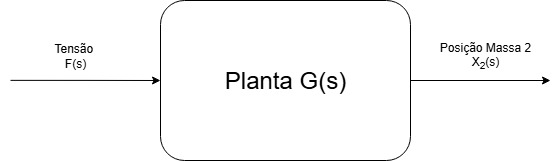
\includegraphics[width = 0.80\columnwidth]{DiagramaFT.jpg}
    \caption{Diagrama de blocos do sistema em malha aberta}
    \label{DiagramaFT}
\end{figure}

\subsection{Consideração sobre a Gravidade}

Para a configuração vertical, a força de gravidade ($F_G = M \cdot g$) atua constantemente em ambas as massas. Este efeito é responsável por estabelecer a posição de equilíbrio estático do sistema, ou seja, a gravidade estica as molas até um novo ponto de repouso. O modelo dinâmico e as EDOs foram desenvolvidas para deslocamentos ($x_1(t)$ e $x_2$(t)) a partir deste ponto de equilíbrio. Como a força da gravidade é constante, ela é cancelada pelas forças estáticas das molas no ponto de equilíbrio, e por isso o termo \textbf{g} não aparece na função de transferência dinâmica.

\begin{figure}[H]
    \centering
    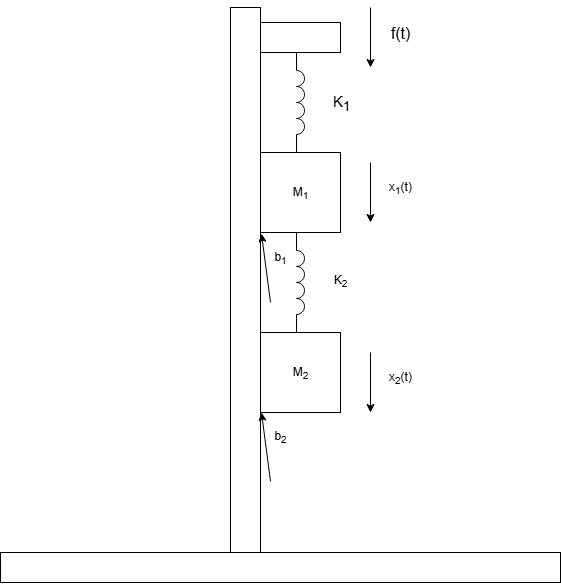
\includegraphics[width=0.80\columnwidth]{DiagramaForca.jpg}
    \caption{Modelagem do sistema massa-mola}
    \label{fig:MSM}
\end{figure}

%Criar um diagrama de blocos simples com uma entrada Y(s), um bloco contendo G(s) e uma saída X2(s)

\section{Análise do Modelo}

A estabilidade do sistema em malha aberta é determinada pelos polos da função de transferência, que são as raizes do polinômio característico do denominador:
\begin{equation}
    \Delta (s) = (M_1s^2 + b_1s + K_1 + K_2)(M_2s^2 + b_2s + K_2) - K_2^2 = 0
\label{eq:raizes}
\end{equation}

Como o polinômio característico agora é um polinômio de quarta ordem completo, com termos de todas as potências de s. Consequentemente, para quaisquer valores físicos positivos dos parâmetros (M, b, K), os polos da função de transferência possuirão parte real negativa, deslocando-se do eixo imaginário para o semiplano esquerdo do plano s.

Isso garante que o sistema em malha aberta seja estável. O comportamento dinâmico esperado para uma entrada degrau é, portanto, uma resposta oscilátoria amortecida, na qual o deslocamento da massa converge para um valor de regime estacionário após um período transitório. A localização exata dos polos e, por conseguinte, as características da resposta transitória -- como a frequência de oscilação amortecida e o tempo de acomodação -- dependem dos valores numéricos de todos os parâmetros físicos do sistema ($M_1, M_2, b_1, b_2, K_1, K_2$).

\section{Simulação Computacional}

Para validar o comportamento dinâmico previsto pelo modelo matemático, foi realizada uma simulação computacional utilizando o software MATLAB/Simulink.

Para a simulação, foram adotados valores preliminares para as constantes das molas, baseados em componentes comerciais comuns (ex: $K_1 = 100N/m$ e $K_2 = 150N/m$). É importante ressaltar que estes valores serão substituídos pelos valores reais medidos.

\begin{figure}[H]
    \centering
    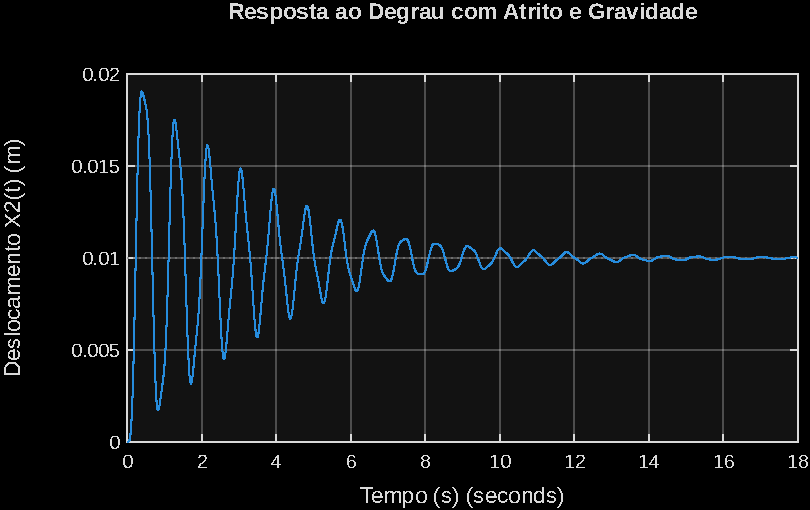
\includegraphics[width=0.75\columnwidth]{RespostaDegrauGravidade.pdf}
    \caption{Resposta ao Degrau}
    \label{fig:RDG}
\end{figure}

\begin{figure}[H]
    \centering
    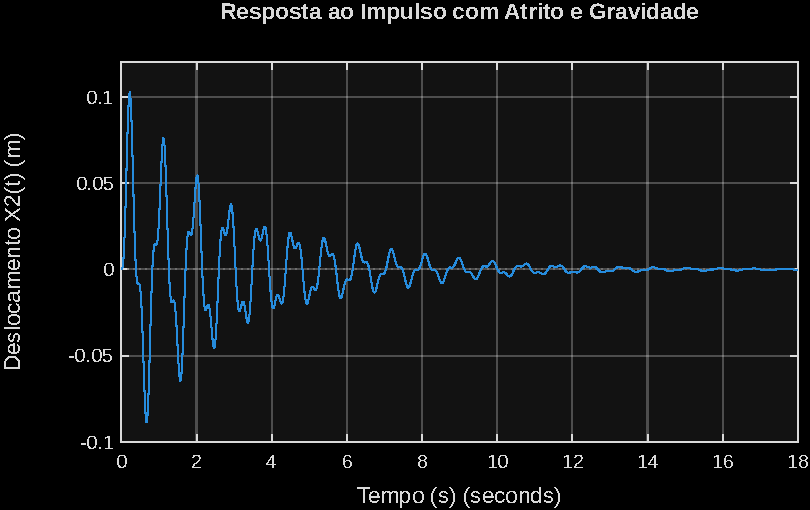
\includegraphics[width=0.75\columnwidth]{RespostaImpulsoGravidade.pdf}
    \caption{Resposta ao Impulso}
    \label{fig:RIG}
\end{figure}

%simulação do MATLAB, gerar gráfico da resposta ao degram e ao impulso e inseri-los

\subsection{Análise dos Resultados da Simulação}
Os resultados da simulação, apresentados nas Figuras \ref{fig:RDG} e \ref{fig:RIG}, confirmam visualmente a análise teórica do modelo desenvolvido. A resposta ao degrau (Figura \ref{fig:RDG}) exibe o comportamento característico de uma oscilação amortecida, onde o sistema, após um transitório oscilatório, converge para um valor de regime estacionário de aproximadamente 0.01 m. A presença de um sobressinal e a subsequente atenuação da amplitude das oscilações são consistentes com um sistema estável de ordem superior, como previsto.

De forma análoga, a resposta ao impulso (Figura \ref{fig:RIG}) mostra o sistema sendo deslocado de sua posição de equilíbrio e retornando a ela de forma oscilatória e amortecida, até cessar o movimento. A convergência em ambos os casos valida o caráter estável do sistema previsto pelo modelo que inclui os efeitos do atrito.

\section{Conclusão Parcial}

 A presente etapa do projeto culminou no desenvolvimento e simulação de um modelo matemático para o sistema de duas massas com acoplamento flexível. Foi obtida uma função de transferência que incorpora os parâmetros físicos do sistema, incluindo as massas, constantes elásticas e coeficientes de atrito, prevendo corretamente a natureza estável e de oscilação amortecida do sistema. A simulação computacional validou este comportamento dinâmico, fornecendo uma base sólida para a continuidade do projeto.

 O modelo agora verificado servirá como referência para a próxima etapa, que consistirá na montagem do protótipo fisíco e na sua validação experimental. O objetivo será determinar os parâmetros reais do sistema construído e comparar sua resposta a um sinal de entrada com os resultados simulados.



\printbibliography

%----------------------------------------------------------

\end{document}
